Nous décrivons l'architecture logicielle d'un pair, \ie d'une instance de l'application \ac{MUTE} dans un navigateur, dans la \autoref{fig:architecture-log-mute}.

\begin{figure}[!ht]
  \centering
  \includegraphics[page=2, trim=0cm 0cm 0cm 0cm, clip, width=.7\linewidth]{img/mute-figures.pdf}
  \caption{Architecture logicielle de l'application MUTE}
  \label{fig:architecture-log-mute}
\end{figure}

Cette architecture logicielle se compose de plusieurs composants, que nous regroupons par couche.
Chacune de ces couches possède un rôle, que nous présentons brièvement ci-dessous avant de les décrire de manière plus détaillée dans leur section respective.
\begin{enumerate}
    \item La couche \emph{interface utilisateur}, qui regroupe l'ensemble des composants permettant de communiquer des informations aux pairs et avec lesquelles ils peuvent interagir, \ie le document lui-même, son titre mais aussi la liste des collaborateur-rices actuellement connectés.
        Cette couche se charge de transmettre les actions de l'utilisateur-rice aux couches inférieures, et inversement de présenter à l'utilisateur-rice les modifications effectuées par ses pairs.
    \item La couche \emph{réplication}, qui regroupe l'ensemble des composants permettant de représenter les données répliquées entre pairs, \ie les \acp{CRDT} utilisés pour représenter le document, ses métadonnées (titre, date de création...), l'ensemble des collaborateurs et leur curseur.
        Cette couche se charge d'intégrer les modifications effectuées par l'utilisateur-rice et de transmettre les opérations correspondantes aux couches inférieures, et inversement d'intégrer les opérations effectuées par ses pairs et d'indiquer à la couche \emph{interface utilisateur} les modifications correspondantes.
    \item La couche \emph{livraison}, qui est constitué d'un unique composant permettant de garantir les modèles de livraison requis par les différents \acp{CRDT} implémentés pour représenter le document.
        Cette couche se charge d'adjoindre aux opérations de l'utilisateur-rice leur(s) dépendance(s) avant de les transmettre aux couches inférieures, et de livrer les opérations de ses pairs une fois leur(s) dépendance(s) livrées au préalable, ou de les mettre en attente le cas échéant.
    \item La couche \emph{sécurité}, qui est constitué d'un unique composant gérant le chiffrement des messages.
        Cette couche se charge d'établir la clé de chiffrement de groupe, puis de chiffrer les messages de l'utilisateur-rice avec cette dernière avant de les transmettre à la couche inférieure, et inversement de déchiffrer les messages chiffrés de ses pairs avant de les transmettre aux couches supérieures.
    \item La couche \emph{réseau}, qui est constitué d'un unique composant permettant d'interagir avec le réseau \ac{P2P}.
        Cette couche se charge d'établir les connexions \ac{P2P}, puis permet de diffuser les messages chiffrés de l'utilisateur-rice à un ou plusieurs de ses pairs, et inversement de transmettre les messages chiffrés de ses pairs à la couche supérieure.
\end{enumerate}

